\documentclass{InsightArticle}

\usepackage[dvips]{graphicx}
\usepackage{float}
\usepackage{subfigure}

\usepackage[dvips,
bookmarks,
bookmarksopen,
backref,
colorlinks,linkcolor={blue},citecolor={blue},urlcolor={blue},
]{hyperref}

\title{Object Boundary Determination and Approximation}

% 
% NOTE: This is the last number of the "handle" URL that 
% The Insight Journal assigns to your paper as part of the
% submission process. Please replace the number "1338" with
% the actual handle number that you get assigned.
%
\newcommand{\IJhandlerIDnumber}{3250}

% Increment the release number whenever significant changes are made.
% The author and/or editor can define 'significant' however they like.
\release{0.00}

% At minimum, give your name and an email address.  You can include a
% snail-mail address if you like.

\author{David Doria}
\authoraddress{Rensselaer Polytechnic Institute, Troy NY. Army Research Laboratory, Aberdeen MD}


\begin{document}

\IJhandlefooter{\IJhandlerIDnumber}


\ifpdf
\else
   %
   % Commands for including Graphics when using latex
   % 
   \DeclareGraphicsExtensions{.eps,.jpg,.gif,.tiff,.bmp,.png}
   \DeclareGraphicsRule{.jpg}{eps}{.jpg.bb}{`convert #1 eps:-}
   \DeclareGraphicsRule{.gif}{eps}{.gif.bb}{`convert #1 eps:-}
   \DeclareGraphicsRule{.tiff}{eps}{.tiff.bb}{`convert #1 eps:-}
   \DeclareGraphicsRule{.bmp}{eps}{.bmp.bb}{`convert #1 eps:-}
   \DeclareGraphicsRule{.png}{eps}{.png.bb}{`convert #1 eps:-}
\fi


\maketitle


\ifhtml
\chapter*{Front Matter\label{front}}
\fi

\begin{abstract}
\noindent

This document presents an implementation of an algorithm to find a low vertex-count polygonal approximation of the outline of a set of 2D points which describe an object homeomorphic to a disc (i.e. without holes).

This implementation is based on the algorithm described in \cite{WangThesis} and \cite{WangPaper}.

The code is available here:
https://github.com/daviddoria/BoundingPolygon

\end{abstract}

\IJhandlenote{\IJhandlerIDnumber}

\tableofcontents
%%%%%%%%%%%%%%%%%%%%
\section{Introduction}
This document presents an implementation of an algorithm to find a low vertex-count polygonal approximation of the outline of a set of points. The input is a 2D point cloud of a solid 2D object. Our goal is to represent the outline of this object in a simple fashion. This type of algorithm is commonly found in applications involving building detection from aerial LiDAR data. However, it can also be used in a more general setting. It is often useful to create a closed contour froma set of points describing the outline of an organ in a medical image processing application. When the convex hull is a poor representation, this technique could be used to find a reasonable closed path through the points. 

This implementation is based on the algorithm described in \cite{WangThesis} and \cite{WangPaper}.

%%%%%%%%%%%%%%%%%%%%
\section{Algorithm Input}
\label{sec:AlgorithmInput}
The core of the algorithm operates on a point cloud describing only the outline of an object. Because of this, the input could take two forms. First, the input could be the coordinates of the edge pixels from an edge image of the object. In this case, these edge point coordinates are exactly the point cloud describing the object outline. In Figure \ref{fig:EdgeImage}, we show a simple data set consisting of a brown rectangular object on a green background. The edge image was produced using itkGradientMagnitudeImageFilter followed by itkThresholdImageFilter.

\begin{figure}[H]
\centering
\subfigure[A brown rectangular object.]
  {
  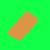
\includegraphics[width=0.3\linewidth]{images/rectangleSolid}
  \label{fig:EdgeImage:Image}
  }
\subfigure[A simple edge pixel classification. White pixels are edge pixels.]
  {
  
\includegraphics[width=0.3\linewidth]{images/rectangleSolidEdgeThresholded}
  \label{fig:EdgeImage:EdgeImage}
  }
\caption{An image of an object and its corresponding edge image.}
\label{fig:EdgeImage}
\end{figure}

In other cases, we will have a point cloud describing the entire object, not just its boundary. In that case, we must perform a preprocessing step (Section \ref{sec:BoundaryPointDetection}) to determine the boundary points before proceeding with the polygonal outline approximation. In Figure \ref{fig:SolidPointCloud} we show a synthetic example of such a data set.

\begin{figure}[H]
  \centering
  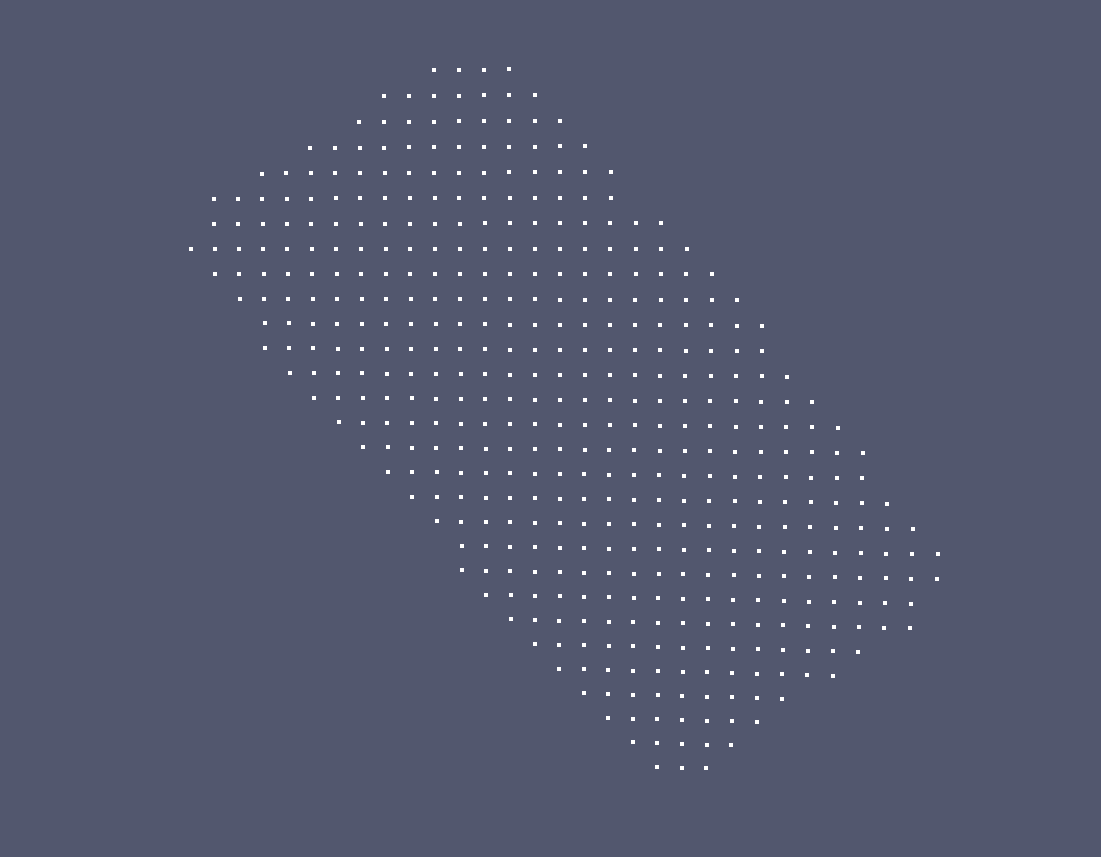
\includegraphics[width=0.3\linewidth]{images/rectanglePoints}
  \caption{A solid point cloud of a rectangular 2D object.}
  \label{fig:SolidPointCloud}
\end{figure}

%%%%%%%%%%%%%%%%%%%%
\section{Optional Preprocessing - Boundary point detection}
\label{sec:BoundaryPointDetection}
If our data set is an object described by a solid 2D point cloud, we must first determine which points are on the boundary of the point cloud. Each point is determined to be on the bounary or not based only on its local neighborhood.  We utilize the fact that boundary points, by definition, do not have any neighbors in a large angular section of their neighborhood. Each point is classified using the following procedure:

\begin{itemize}
 \item For each point $p$, find its neighbors $n_i$ within a radius $R$. We use a KD-Tree to efficiently perform the neighborhood search computation.
 \item Determine the angle formed by the vector between $p$ and each $n_i$. These angles are found using the arctangent (i.e. $\theta_i = atan2(n_{i_x} - p_x, n_{i_y} - p_y)$ ), so they are s measured from the standard mathematical reference vector $(1,0)$. 
 \item Sort the vectors by their angles, as the neighbors were not found in any particular anglular order.
 \item Compute the angle between each adjacent ordered vector. This is simply the difference of the angles formed by two adjacent vectors. Be sure to use the interior angle - that is, if the angle difference computed is greater than 180 degrees, subtract the difference from 360. For example, if the two angles are 350 and 10, the difference should be 20.
 \item If the difference between any two adjacent vectors is greater than a threshold (we typically use 70 degrees as the threshold), the point is declared to be a boundary point. 
\end{itemize}

In Figure \ref{fig:BoundaryDetermination}, we show a point which should be classified as a boundary point.

\begin{figure}[H]
\centering
\subfigure[A zoomed out view of a neighborhood for context.]
  {
  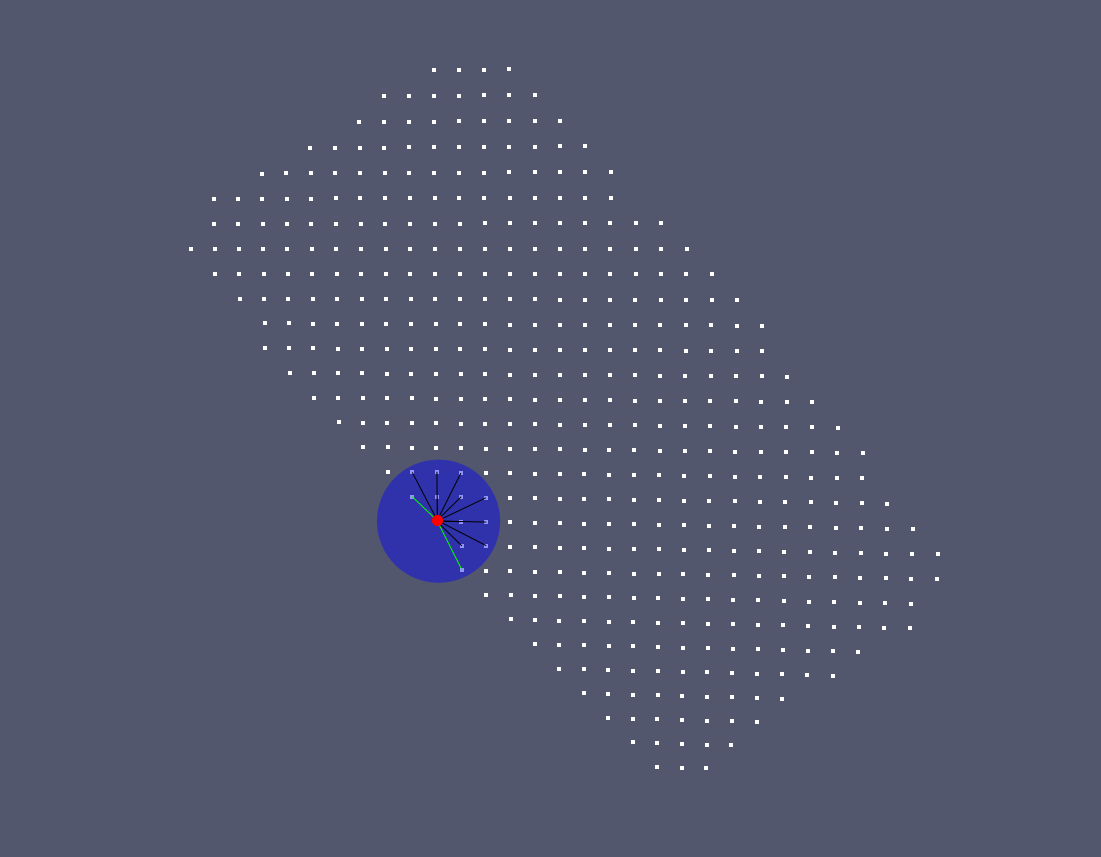
\includegraphics[width=0.3\linewidth]{images/boundaryDetermination}
  \label{fig:BoundaryDetermination:ZoomedOut}
  }
\subfigure[A point and its neighborhood.]
  {
  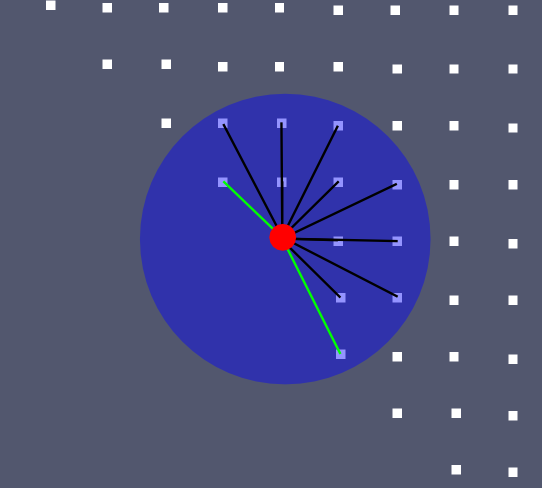
\includegraphics[width=0.3\linewidth]{images/boundaryDeterminationZoomed}
  \label{fig:BoundaryDetermination:ZoomedIn}
  }
\caption{Graphical representation of the process used to determine if a point is on the boundary. The red point is the query point. The blue circle is radius $R$ and encloses some neighboring points. The black lines are vectors from the query point to neighboring points. The green lines represent the vectors with an angular separation greater than the specified threshold of 70 degrees.}
\label{fig:BoundaryDetermination}
\end{figure}

%%%%%%%%%%%%%%%%%%%%
\section{Boundary Polygonal Approximation}
\label{sec:PolygonalApproximation}
The input to this part of the algorithm is a set of points describing the outline of the object. These points will typically be very noisy, either from the acquisition process itself, noise in the acquisition, or error in the boundary point computation or edge detection and thresholding, depending on the type of input data.

\subsection{Rough Boundary Approximation}
We must first form a rough closed loop on the data points. It is acceptable if some points are not included, and it is also acceptable if the boundary contour is self intersecting, but it is critical that the path along the boundary is a closed loop. To find such a contour, we use the following procedure:

\begin{itemize}
 \item Select any point (at random) from which to start.
 \item Find the nearest neighbor to the current point from the set of points that has not already been added to the path and add it to the path. We use a KDTree for computational efficiency.
\end{itemize}

Figure \ref{fig:RoughBoundary} shows a case where this method works very well. You can see how the noise is followed exactly. This boundary consists of 41 line segments, where one could imagine the rectangular object being represented with only 4.
\begin{figure}[H]
\centering
\subfigure[The boundary points of a rectangular object.]
  {
  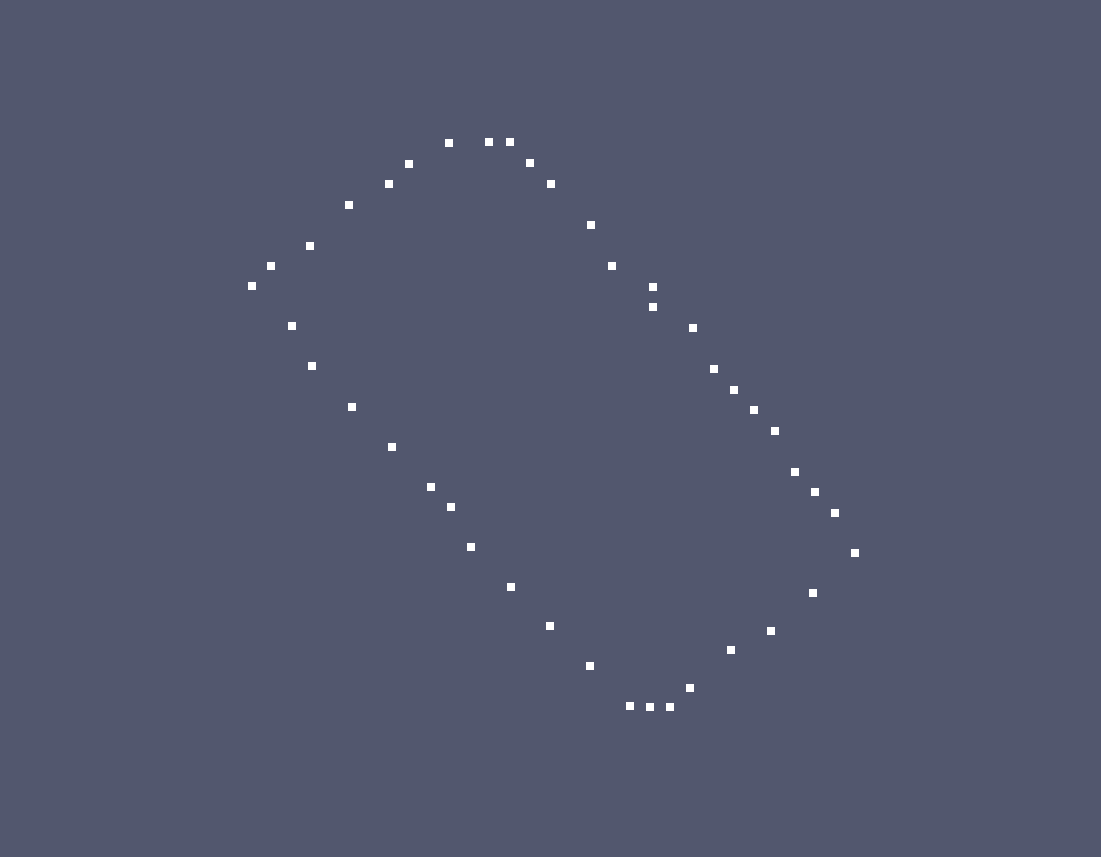
\includegraphics[width=0.3\linewidth]{images/rectangleRoughPoints}
  \label{fig:RoughBoundary:Points}
  }
\subfigure[The rough path found on the boundary points.]
  {
  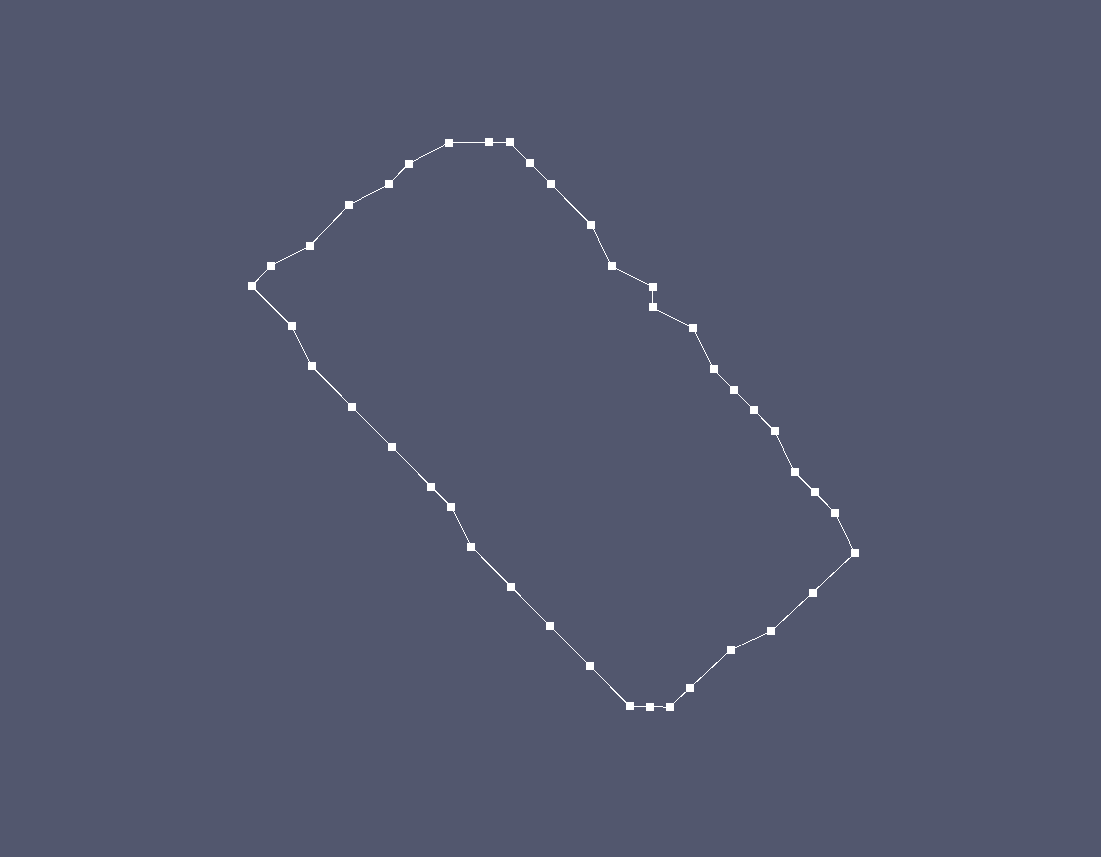
\includegraphics[width=0.3\linewidth]{images/rectangleRoughPath}
  \label{fig:RoughBoundary:Path}
  }
\caption{The rough path computed for a rectangular objects bounding points.}
\label{fig:RoughBoundary}
\end{figure}

As demonstrated in Figure \ref{fig:RoughBoundary}, for very low noise, sufficiently dense input data, this procedure works very well. However, in data sets with noise or too few samples in some regions, points may be skipped, which is acceptible. However, often the loop will not be closed before one of these skipped points is the closest non-added point, and a failure case occurs.


\subsection{Boundary Simplification}
Once we have a reasonable closed loop around the points, it is often very noisy. It is often desirable to reduce the data to a simple model. For example, in the case of building detection, we often want to represent a building as a rectangle (4 line segments). Depending on the density of the input, the boundary at this point could be represented by hundreds of line segments, mostly describing the noise. To reduce the number of line segments in the boundary, we use the following procedure:
\begin{itemize}
 \item Create a directed graph of the contour using exactly the vertices of the rough boundary as the vertices and the ordered line segments of the rough boundary as directed edges.
 \item Attempt to add every other possible edge (from each vertex to every other vertex ahead of it in the contour ordering) only if the new edge passes a straightness test.
 \item The straightness test is described in \cite{WangThesis} as the sum of the distances from every point between the two end points to the proposed edge. We have found it more convenient to set this threshold based on the average of these distances, as the length of the edges then is not a factor in determining the straightness criteria.
\begin{figure}[H]
  \centering
  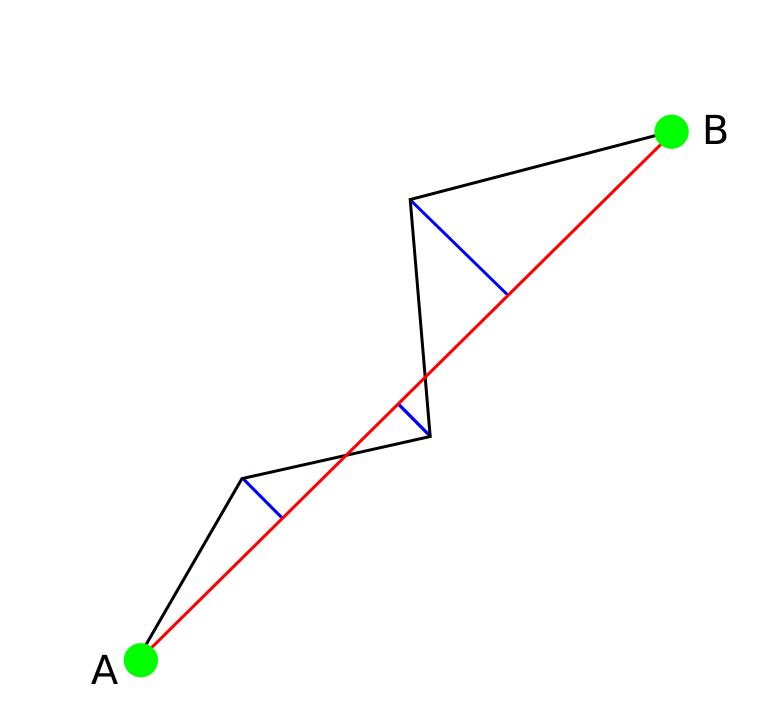
\includegraphics[width=0.3\linewidth]{images/straightness}
  \caption{The straightness computation of a proposed edge between vertices A and B. Black: the rough boundary. Red: the proposed edge. Blue: the distances from all points on the boundary between A and B to the proposed edge.}
  \label{fig:Straightness}
\end{figure}
 \item By finding any full loop shortest path on this graph, we will have significantly improved (i.e. reduced the line count of) our boundary. However, it is not a well posed graph theoretic problem to ask for the shortest path from a vertex to itself (a loop) and expect a non-zero answer (i.e. the shortest path from a vertex to itself is to not move at all!). To remedy this, we add the ordered vertices around the boundary twice, as well as duplicate the edges on this second loop of vertices. Now we can ask for the shortest path from vertex $i$ to vertex $i+N$ where $N$ is the original number of vertices in the rough boundary.
 \item If we compute this shortest path from any random vertex, we will have a solution to our original problem of finding a low-line segment count approximation to the boundary. However, the choice of starting vertex actually can change the solution, though often only slightly. Because of this, we find the shortest path starting at all vertices, and choose the shorest one as our solution.
\end{itemize}

[Demonstrate the case where the starting point is not on the best shortest path. This is why we must find all shortest paths from all points, not just one.]

%%%%%%%%%%%%%%%%%%%%
\section{Demonstration}
\label{sec:Demonstration}

% \begin{figure}[H]
% \centering
% \subfigure[Image to be filled. The region to be filled is shown in bright green.]
%   {
%   \includegraphics[width=0.3\linewidth]{images/BlackWhite}
%   \label{fig:SyntheticDemonstration:ExampleInputImage}
%   }
% \subfigure[The mask of the region to inpaint.]
%   {
%   \includegraphics[width=0.3\linewidth]{images/BlackWhiteMask}
%   \label{fig:SyntheticDemonstration:ExampleInputMask}
%   }
% \subfigure[The result of the inpainting.]
%   {
%   \includegraphics[width=0.3\linewidth]{images/BlackWhiteResult}
%   \label{fig:SyntheticDemonstration:ExampleInputOutput}
%   }
% \caption{Synthetic Demonstration}
% \label{fig:SyntheticDemonstration}
% \end{figure}

%%%%%%%%%%%%%%%
\section{Code Snippet}

\begin{verbatim}

\end{verbatim}

%%%%%%%%%%%
\section{Future Work}
There are several parameters throughout these algorithms. In the boundary point detection, there is the radius of the nearest neighbor search and the angle at which to declare a point on the boundary. In the polygonal approximation, there is a minimum straightness parameter which must be set. Removing the need to manually specify these parameters would making these algorithms more robust to different data types, as well as provide the best possible results on any particular data set.

%%%%%%%%%%%%%%%
\begin{thebibliography}{9}

	\bibitem{WangThesis}
	  Wang, O.,
	  \emph{Using Aerial Lidar Data to Segment And Model Buildings}.
	  University Of California Santa Cruz Masters Thesis, 2006


	\bibitem{WangPaper}
	  Wang. O, Lodha. S, Helmbold, D.,
	  \emph{A Bayesian Approach to Building Footprint Extraction from Aerial LIDAR Data}.
	  3D Data Processing, Visualization, and Transmission 2006

\end{thebibliography}

\end{document}